\chapter{Hintergrund}
\label{chap:background}

Die Grundlagen stellen ein gemeinsames Verständnis zur Auswahlkomponente her.
Dazu zählen die Zustände, welche in diesem Zusammenhang auftreten können.
Ausserdem behandelt es eine Basis zu den Themen Browser und Rendering. 
Dieses Verständis ermöglicht es, eine neue, konsistente Komponente zu entwickeln.


\section{Ausgangslage}
\label{sec:basics}

Studenten als auch Mitarbeiter entwickeln das Toolkit Kolibri laufend weiter.
Entwickler können die Open Source Werkzeuge ganz einfach importieren und verwenden.
Damit das Kolibri-Toolkit schlank bleibt, kommen keine externen Abhängigkeiten zur Verwendung.
Mit einer VanillaJS Codebasis bietet das Tool eine breite Auswahl an, deckt aber noch nicht alle Interaktionen ab.

In diesem Projekt dient der in der Vorarbeit erstellte Fork als Ausgangslage.
Ein Merge – des Branches \emph{experimental} dieses Forks und des \emph{Kolibri-16} der originalen Codebasis – stellt die Aktualität sicher.
Das \codestyle{SimpleInput} ist eines der Tools, welches sich bei der Implementation der neuen Auswahlkomponente als hilfreich erweisen kann.

Der Zugriff auf das Tool Figma ermöglicht das Verwenden des existierenden Designsystems und der bereits eingebundenen Elemente. 
Der Aufbau der Elemente als Komponenten vereinfacht die Wiederverwendung. 
Das Ergänzen des Icon-Sets ist bei Bedarf erlaubt.

Eine weitere, wichtige Ausgangslage ist ein gemeinsames Verständnis der verwendeten Begriffe. 
Dies sicherzustellen ist die Aufgabe des nächsten Kapitels mit der Beschreibung der Zustände einer Auswahlkomponente als auch derer Elemente.
Diese Definitionen gelten im gesamten Bericht.


\section{Zustände in einer Auswahlkomponente}
\label{sec:states}

Dieser Abschnitt erklärt die Zustände, welche in einer Auswahlkomponente auftreten können.
Als Ausgangslage dient eine Eingabemöglichkeit, die eine Master-Detail-Ansicht\footnote{
    Master beschreibt den Bereich, welcher alle möglichen Auswahlwerte enthält. 
    Detail beschreibt den Bereich, welcher den aktuell ausgewählten (selektierten) Wert enthält.
} aufweist.
Zudem sind keine speziellen Voreinstellungen getroffen.

Je nach Darstellung der Komponente kann diese \emph{offen} oder \emph{geschlossen} sein.
Wenn nur einer der beiden Zustände möglich ist, ist es meistens der Offene.
Im geschlossenen Status zeigt das Erscheinungsbild nur die Detail-Ansicht an, welcher mindestens den selektierten Wert anzeigt.
Eine offene Auswahlmöglichkeit stellt beide Elemente der Master-Detail-View dar.
Die Master-Ansicht zeigt alle Values einer Liste an.

Bei dem \emph{normalen} bzw. nicht fokussierten Status ist die Komponente nicht an- oder ausgewählt.
Wenn eine Webseite diese Komponente enthält, ist dies die standardmässige Darstellung.
Das neue Element zeigt keine Reaktion auf Interaktionen, welche in diesem Zustand geschehen. 
Als einzige Ausnahme gilt Tab, welche den Fokus auf die Komponente legen kann. 
In den meisten Erscheinungen ist nur die Detail-Ansicht sichtbar und der Master-Container ist ausgeblendet.
Wählt der Nutzer die Komponente mit der Maus oder der Tastatur an, steht sie im \emph{Fokus} bzw. ist sie \emph{fokussiert}.
Bedienungen über das Keyboard beziehen sich hierbei auf den Baustein.
In den meisten Fällen ändert sich die Darstellung des Eingabefeldes z.B. durch einen blauen Rahmen.

Ist ein Wert in der Master-Ansicht ausgewählt und erscheint in der Detail-View, ist dieser \emph{selektiert}.
Das Formular enthält beim Versenden das Value der \emph{Selektion}.
Eine \emph{Selektion} in einer Kategorie-Spalte findet in den Formulardaten keine Berücksichtigung.
Stattdessen filtert die Kategorie-Selektion die Wert-Spalte.
Durch das Hervorheben zeigt sich in der Liste aller Werte eine getätigte Auswahl an.
In gewissen Situationen existiert noch der Zustand, dass in der Master-View ein Wert im \emph{Highlight} steht. 
Bestätigt der Nutzer das \emph{Highlight} mit der Maus, wechselt der Status auf selektiert.
Das Hovern kann den Highlight-Wert ändern. 
Geschieht die Navigation durch die Werte mit der Tastatur, erhält genau ein Wert die \emph{Cursor Position}. 
Durch das Betätigen gewisser vordefinierter Tasten ändert sich die \emph{Cursor Position}.
Bei einer Bestätigung mit der Tastatur ändert sich der Wert der \emph{Cursor Position} auf selektiert.
Die letzten zwei Zustandswerte haben keinen Einfluss auf das versendete Formular und sind nur im Master zu finden.
Nachfolgend sind noch die Details zum Thema Browser erklärt.


\section{Browser \& HTML Renderer}
\label{sec:browserRenderer}

Die wichtigsten Aspekte von der Theorie über die populären Browser bis hin zum Ablauf des Renderings sind hier aufgeführt.
Dabei sind nur die bekanntesten Implementationen von Belang.

Ein Webbrowser dient als Zugang ins Internet und zur Anzeige von Webressourcen wie HTML, CSS und JavaScript.
Er besteht aus einer Benutzeroberfläche, einer Browser- und einer Rendering-Engine.
Für eine verständliche Darstellung der Inhalte auf dem UI verwendet die Browser-Engine einen sogenannten Renderer - mehr dazu später.
Die Benutzeroberfläche dient als Schnittstelle zwischen dem Benutzer und der Datenschicht. 
Die Rendering-Engine interpretiert die Inhalte anhand des vorgegebenen Inhaltstyps. 
Einer der Engines ist der HTML-Renderer.
Beim UI und der Bedienung zeigen sich die Uneinigkeiten zwischen den Browser-Herstellern, indem die Rendering-Engine den Code nicht gleich interpretiert.
Anschliessend sind Informationen über den detaillierten Ablauf zur Anzeige eines HTML-Dokuments und die Rolle des Rendering dokumentiert.


\subsection{Rendering Prozess}
\label{sec:structureRendering}

Der Aufruf einer Webseite beginnt mit dem HTTP-Request auf welchen eine HTTP-Response folgt.
In diesem Bericht sind die gerade genannten Schritte vor dem eigentlichen erhalten der Daten nicht weiter wichtig.
Der Response liefert schlussendlich die anzuzeigenden Daten, welche in diesem Fall die tragende Rolle spielen.

\begin{figure}[!htb]
    \centering
    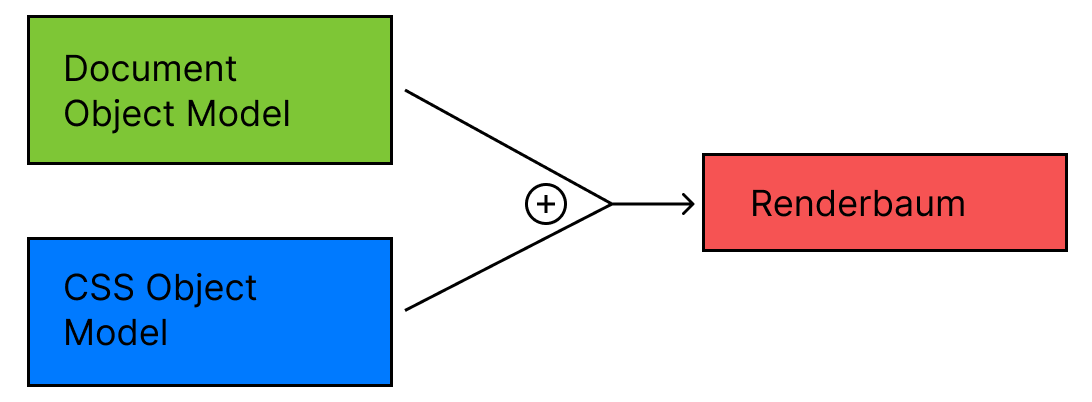
\includegraphics[width=80mm]{rendering-process.png}
    \caption{Rendering Prozess}
    \label{img:renderingProcess}
\end{figure}

Der Browser verarbeitet die erhaltenen Daten im HTML-Format weiter.
Mehrere Schritte wandeln die einzelnen HTML-Elementen in sogenannte Nodes um. 
Aus den resultierenden Nodes entsteht durch Verknüpfungen eine Baumstruktur - der DOM.
Das Document Object Model (DOM) (Abbildung \ref{img:renderingProcess} links oben) beschreibt die Eltern-Kind- und Geschwister-Beziehung der Nodes.
Der Prozess bis zum CSS Object Model (CSSOM) gestaltet sich relativ ähnlich, ist aber nicht weiter wichtig.

Der DOM und der CSSOM sind unabhängig von einander. 
Der Browser kombiniert die beiden Bäume zu einem gemeinsamen Renderbaum (Abbildung \ref{img:renderingProcess} rechts).
Der resultierende Baum repräsentiert nur sichtbare Elemente, wohingegen der DOM alle Elemente enthält.
Der Renderbaum ist browserabhängig.

Dieses Wissen ist wichtig für das spätere Kapitel \textbf{\nameref{sec:performance}}. 
Der Grund ist, dass der Browser maximal 60 Mal pro Sekunde rendern kann.
Jede Änderung am Browser-DOM\footnote{
    Im Renderbaum verwendeter und im Browser angezeigter DOM
} startet den kompletten Rendering Prozess von vorne.
Zu viele Änderungen am DOM führen dazu, dass der Nutzer länger warten muss, bis die Webseite geladen ist.

Gründe für ein erneutes Rendern\citemarktext{
    [\cite{browserRendering3}]
}:

\begin{itemize}
    \item Manipulation der Elemente des DOM
    \item Änderungen vom Inhalt (auch von Formularfeldern)
    \item Änderungen in den CSS-Eigenschaften
    \item Hinzufügen oder Entfernen von Stylesheets
    \item Ändern des Attributs \codestyle{class}
    \item Grössenänderung des Browserfensters
    \item Scrollen
    \item Pseudo-Klassenaktivierung
\end{itemize}


\subsection{Bekannte Implementationen}
\label{sec:implementationsRenderer}

Die neue Komponente soll in möglichst allen Browsern eine konsistente Erscheinung als auch Interaktion bieten.
Durch die Erklärung aus Kapitel \textbf{\nameref{sec:structureRendering}} ist klar, dass die Renderer die Unterschiede im UI bewirken.
Die Bedienungsabweichungen stammen grösstenteils vom zu Grunde liegenden Betriebssystem.
Diese Erkenntnisse führen dazu, dass die neue Komponente auf Mac und Windows in den Browsern der jeweils geläufigsten Rendering-Implementationen zu testen ist.
Zu den ausgewählten Webbrowser zählen Google Chrome, Firefox (Mac und Windows), Safari (nur Mac) und Edge (nur Windows).
Die Erläuterung dazu folgt im nächsten Abschnitt.

Die populärsten Browser mit 65\% Marktabdeckung basieren auf der Chromium-Basis und verwenden alle den HTML-Renderer Blink\citemarktext{
    [\cite{blinkRenderer}]
}.
Die Entwickler dieser Rendering-Engine sind die Open Source Community Chromium, Google, Intel und Samsung.
Zu den Verwendern\citemarktext{
    [\cite{chromiumBrowser}]
} von Blink zählen unter anderem Google Chrome, Brave, Microsoft Edge, Opera und Vivaldi.
WebKit\citemarktext{
    [\cite{webkitRenderer}]
} – der Vorgänger des geläufigsten Renderer – findet sich im OSX Webbrowser Safari wieder.
Diese von Apple, Google, KDE und Nokia entwickelte Rendering-Engine deckt 15\% ab.
Als bekannester Vertreter des Restes zählt Firefox\citemarktext{
    [\cite{mozillaBrowser}]
} sowie weitere mozilla-basierte Browser, welche die Webseiten mit Gecko renderen.
Es existieren noch weitaus mehr Renderer, welche aber eine sehr geringe Verbreitung aufweisen.
Deswegen sind diese nicht weiter von Belang.
